%==================================================================FRONT PAGE AND TOC
% For article only
\mode<presentation:0>{\thispagestyle{empty}\maketitle}

% For presentation only
\mode<presentation| article:0| handout:0>{
    \begin{frame}<article:0>[label=portada]
    \titlepage
    \end{frame}%Fin del frame
}

% For handout only
\mode<handout>{
  \begin{frame}[label=portada]
    \maketitle
  \end{frame}
}

%% TABLE OF CONTENTS
\begin{frame}[label=toc]
    \mode<article:0>{\frametitle{Contents}}
    \mode<presentation>{\small}
    \tableofcontents[hidesubsections]
\end{frame}

%%==================================================================S INTRODUCTION
\section{What's ALS}
%%==================================================================Sb
\subsection{Principles}
%%==================================================================F 
\begin{frame}[label=lidar]
    \frametitlee{ALS principles}
    \begin{enumerate}
        \item Airborne Laser Scanner (ALS) is given by the combination of:
	\uncover<1->{
	\begin{itemize}
	 \item \alert<1>{Laser scanner}
	 \item \alert<1>{GPS} which provides the location of the sensor
	 \item \alert<1>{INS} which provides its orientation parameters: pitch, roll and yaw
	\end{itemize}
	}
	\uncover<2->{
	\item The relative position of the reflecting ground spot with respect to the laser scanner emission point is determined by:
	\begin{itemize}
	 \item The \alert<2>{time} each pulse takes to reach the ground and return back
	 \item The \alert<2>{angle} from the nadir at which it has been emitted
	\end{itemize}
	}
	\uncover<3->{\item The laser data are then combined with the sensor location and orientation to give the \alert<3>{coordinates X, Y, Z (WGS84)} of the laser footprint on the terrain surface.}
    \end{enumerate}
\end{frame}
%%==================================================================F 
\mode<beamer>{
  \pgfdeclareimage[width=100mm]{ray}{images/ray}
  \pgfdeclareimage[width=100mm]{echo}{images/echo}
}
\mode<beamer:0>{
  \pgfdeclareimage[width=100mm]{ray_grey}{images/ray_grey}
  \pgfdeclareimage[width=100mm]{echo_grey}{images/echo_grey}
}
\begin{frame}
  \frametitle{ALS principles}
	\mode<beamer>{
    \begin{center}
	
\begin{tikzpicture}
    	  \uncover<1> {\pgftext[bottom,left,at={\pgfpointxy{0}{0}}]{\pgfuseimage{ray}};}
    	  \uncover<2> {\pgftext[bottom,left,at={\pgfpointxy{0}{0}}]{\pgfuseimage{echo}};}
	\end{tikzpicture}
   \end{center}
	}
%	\mode<beamer:0>{
%    \begin{center}
%	\begin{tikzpicture}
%    	  \pgftext<1>[bottom,left,at={\pgfpointxy{0}{0}}]{\pgfuseimage{ray_grey}}
%    	  \pgftext<2>[bottom,left,at={\pgfpointxy{0}{0}}]{\pgfuseimage{echo_grey}}
%	\end{tikzpicture}
%   \end{center}
%	}
\end{frame}
%%==================================================================Sb
\subsection{Characteristics}
%%==================================================================F
\begin{frame}[label=lidar_charact]
    \frametitle{ALS characteristics}
    \begin{enumerate}
    	\item High \alert{accurate measurements} in both altimetric and planimetric components
    	\item Laser pulses are emitted with high repetition rates per second, thus \alert{high resolution} can be obtained.
    	\item \alert{Monoscopy} and \alert{almost-nadirality} permit to reach the ground or the studied object surface even in highly vegetated zones
\end{enumerate}
\end{frame}
%%==================================================================Sb
\subsection{First and Last pulses}
%%==================================================================F 
\mode<beamer>{
  \pgfdeclareimage[height=50mm]{roof}{images/roof}
  \pgfdeclareimage[height=50mm]{tree}{images/tree}
}
\mode<beamer:0>{
  \pgfdeclareimage[height=50mm]{roofg}{images/roof_grey}
  \pgfdeclareimage[height=50mm]{treeg}{images/tree_grey}
}
\begin{frame}[label=firstlast1]
    \frametitle{First and Last pulses}
    \begin{enumerate}
        \item Due to spot size, some pulse may be partially reflected by object at different heights and partially by the terrain. 
	\item The sensor collects at least two (up to several) returns for a single pulse emitted.
    \end{enumerate}
   \begin{center}
   	\begin{tikzpicture}
	\mode<beamer>{
    	  \pgftext[bottom,left,at={\pgfpointxy{-2}{0}}]{\pgfuseimage{roof}}
    	  \pgftext[bottom,left,at={\pgfpointxy{2}{0}}]{\pgfuseimage{tree}}
	}
	\mode<beamer:0>{
    	  \pgftext[bottom,left,at={\pgfpointxy{-2}{0}}]{\pgfuseimage{roofg}}
    	  \pgftext[bottom,left,at={\pgfpointxy{2}{0}}]{\pgfuseimage{treeg}}
	}
	\end{tikzpicture}
   \end{center}
\end{frame}
%%==================================================================F 
\begin{frame}[label=firstlast2]
    \frametitle{First and Last pulses}
    \begin{enumerate}
	\item A considerable difference between first and last pulse can be a clue for the presence of an object with different heights (vegetation or edges of objects, such as buildings, cars, transmission lines, etc.)
	\item No chance exists to directly recognize whether a single reflecting point belongs to the bare earth or to an object.
        \item The data recorded as last pulse (the last return of a single pulse) has the greatest probability to detect the ground
    \end{enumerate}
\end{frame}
%%==================================================================S
\section{Filters}
%%==================================================================Sb
\subsection{Definition}
%%==================================================================F
\begin{frame}[label=filter_def]
    \frametitle{ALS filters}
    \begin{enumerate}[<+->]
	\mode<presentation| article:0>{
	\item A point cloud $V = \left\lbrace v=\left(x,a\right) | x \in \mathbb{R}^3, a \in \mathbb{N} \right\rbrace$, treated as a set of attributed points in a three-dimensional space, where bare earth labeled points take 0 values and 1 otherwise, is \alert<1>{filtered} when points labeled as 1 are removed.}
	\mode<article>{
	\item A point cloud $$V = \left\lbrace v=\left(x,a\right) | x \in \mathbb{R}^3, a \in \mathbb{N} \right\rbrace$$, treated as a set of attributed points in a three-dimensional space, where bare earth labeled points take 0 values and 1 otherwise, is \alert<1>{filtered} when points labeled as 1 are removed.}
	\item That is, \alert<2>{\emph{filtering}} is the automatic procedure of differencing bare earth from objects in ALS point clouds
    \end{enumerate}
\end{frame}
%%==================================================================Sb
\subsection{Motivations and first attempts}
%%==================================================================F
\begin{frame}[label=filter_motivation]
    \frametitle{Motivation of filters}
    \begin{enumerate}
	\item ALS point clouds represent the surveyed surface. Digital Surface Model or \alert{DSM} 
	\begin{itemize}
	 \item Hydrology
	 \item Topography
	 \item Cityscapes 
	 \item Coastal engineering
	 \item Volume computations 
	 \item Power lines
	\end{itemize}
	\item Filtering allows to extract attached (buildings and vegetation) and detached objects (bridges, highpasses,...). Digital Terrain Models or \alert{DTM}
	\begin{itemize}
	 \item Hydrology
	 \item City modelling
	 \item Forestry
	\end{itemize}
    \end{enumerate}
\end{frame}
%%==================================================================F 
\begin{frame}
    \frametitle{First attempts}
    \begin{enumerate}
	\item First version of filter developed by Laboratorio di Geomatica wthin GRASS GIS 5.4
	\begin{itemize}
	  \item s.outlier
	  \item s.edgedeteciton
	  \item s.growing
	  \item s.correction
	  \item s.bspline
	\end{itemize}
	\item Tested in the ISPRS filtering test with good results
    \end{enumerate}
\end{frame}
%%==================================================================Sb 
\subsection{Results}
%%==================================================================F 
\begin{frame}[label=adbpo_results]
    \frametitle{``Autorit\`a del Bacino del Po (Adbpo)'' test}
    \begin{enumerate}
	\item GRASS GIS 5.4 version filter was also used in the Adbpo datasets
	\begin{itemize}
	    \item Coincidence above the 91\% of the points with a manual classification.
	    \item Statistical comparison.
	\end{itemize}
	\begin{table}
	  \begin{center} \resizebox{!}{2cm}{
	    \begin{tabular}{clrrrr}
		\bfseries Zones & \bfseries Models & \bfseries Min  & \bfseries Max & \bfseries Mean & \bfseries RMS \\
		\hline
		\multicolumn{2}{c}{} & \multicolumn{4}{c}{\footnotesize(meters)}\\
		\bottomrule
 		& \small Surface Digital Model & -8.20 & 21.20 & 0.13 & 0.54 \\
 		\textbf{278} & \small Hydraulic without buildings model & -5.20 & 5.50 & 0.07 & 0.27 \\
 		& \small Natural Terrain Model & -5.50 & 5.50 & 0.07 & 0.27 \\
		\hline
 		& \small Surface Digital Model & -11.75 & 18.31 & 0.22 & 0.76 \\
 		\textbf{375} & \small Hydraulic without buildings model & -9.32 & 11.92 & 0.15 & 0.50 \\
 		& \small Natural Terrain Model & -9.32 & 10.58 & 0.14 & 0.48 \\
		\hline
		& \small Surface Digital Model & -12.18 & \alert<2>{41.02} & 0.41 & \alert<2>{1.25} \\
		\textbf{386} & \small Hydraulic without buildings model & -5.14 & 17.24 & 0.24 & 0.72 \\
		& \small Natural Terrain Model & -9.58 & 8.77 & 0.00 & 1.22 \\
		\bottomrule
	    \end{tabular}}
	  \end{center}
	\end{table}
	\item \uncover<2->{\alert<2>{Major problems} arise from vapor clouds and problematic object structures.}
    \end{enumerate}
\end{frame}
%%==================================================================F 
\mode<beamer>{
  \pgfdeclareimage[height=5cm]{fumo}{images/fumo}
}
\mode<beamer:0>{
  \pgfdeclareimage[height=5cm]{fumog}{images/fumo_grey}
}
\begin{frame}
    \frametitle{Adbpo filtering problems}
\begin{table}
  \begin{center} \resizebox{!}{1cm}{
    \begin{tabular}{clrrrr}
	\bfseries Zones & \bfseries Models & \bfseries Min  & \bfseries Max & \bfseries Mean & \bfseries RMS \\
	\hline
	\multicolumn{2}{c}{} & \multicolumn{4}{c}{\footnotesize(meters)}\\
	\bottomrule
	& \small Surface Digital Model & -12.18 & \alert{41.02} & 0.41 & \alert{1.25} \\
	\textbf{386} & \small Hydraulic without buildings model & -5.14 & 17.24 & 0.24 & 0.72 \\
	& \small Natural Terrain Model & -9.58 & 8.77 & 0.00 & 1.22 \\
	\bottomrule
    \end{tabular}}
  \end{center}
\end{table}
   \begin{center}
   	\begin{tikzpicture}
	\mode<beamer>{
    	  \pgftext[bottom,left,at={\pgfpointxy{2}{0}}]{\pgfuseimage{fumo}}
	}
	\mode<beamer:0>{
    	  \pgftext[bottom,left,at={\pgfpointxy{2}{0}}]{\pgfuseimage{fumog}}
	}
	\end{tikzpicture}
   \end{center}
\end{frame}
%%==================================================================S 
\section{Improvements}
%%==================================================================Sb
\subsection{GRASS GIS 6}
%%==================================================================F
\begin{frame}
    \frametitle{Geographic Resources Analysis Support System\hfill \includegraphics[width=0.7cm]{images/grasslogo_transp_big.png}} 
     \begin{enumerate}%[<+->]
	\item Known as \alert<1>{GRASS}, it is a GIS software for the geospatial data management and analysis.
	\item Since is an open source software with lots of built-in libraries, it is possible to implement embedded analysis algorithms.
	\item GRASS 6 vector architecture allows and requires topology (problem to deal with)
	\item It is written in C/C++ that allows to implement heavy computational algorithms
	\item Portable: Version for GNU/Linux, MS-Windows, Mac-OSX, SUN, etc, thus anyone can use it.
	\item More information in:
	\beamergotobutton{\url{http://grass.osgeo.ogr}} 
    \end{enumerate}
\end{frame}
%%==================================================================F
\begin{frame}
    \frametitle{Commands in GRASS GIS 6}
    \begin{enumerate}
        \item Decided to import filtering commands into the new GRASS~GIS~6 vector architecture:
	\begin{itemize}
	    \item s.outlier $\Rightarrow$ {v.outlier}
	    \item s.edgedetection $\Rightarrow$ {v.lidar.edgedetection}
	    \item s.growing $\Rightarrow$ {v.lidar.growing}
	    \item s.correction $\Rightarrow$ {v.lidar.correction}
	    \item s.bspline $\Rightarrow$ {v.surf.bspline}. 
	\end{itemize}
	\item \uncover<2->{Interpolation command (v.surf.bspline) improvements:
	\begin{itemize}
	    \item New \alert<2>{cross validation} algorithm (leave one out)
	    \item New procedure to make interpolation faster (return to ascii files instead of databases)
	\end{itemize}}
	\item \uncover<3->{New vegetation filter: \alert<3>{v.lidar.vegetation}}
    \end{enumerate}
\end{frame}
%%==================================================================Sb
\subsection{Interpolation}
%%==================================================================F
\pgfdeclareimage[height=4cm]{slopee}{images/slope_errors}
\begin{frame}
    \frametitle{Overlapping}
    \begin{enumerate}
	\item During interpolation the whole region is divided in overlapped tiles
	\begin{itemize}
	   \item Make interpolation faster
	   \item Avoid memory allocation problems
	\end{itemize}
	\item A weighted average is computed in the overlapped zones. 
	\begin{itemize}
	   \item Allows the continuity in the whole interpolation
	   \item Introduce a bad behavior in \emph{aspect} maps due to data gaps
	\end{itemize}
    \end{enumerate}
    \begin{center}
       \begin{tikzpicture}
        \pgftext[bottom,left,at={\pgfpointxy{0}{0}}]{\pgfuseimage{slopee}}
       \end{tikzpicture}
    \end{center}
\end{frame}
%%==================================================================F
\pgfdeclareimage[height=7cm]{tiles}{images/tiles}
\pgfdeclareimage[height=7cm]{slopef}{images/slope_features}
\pgfdeclareimage[height=7cm]{slopefp}{images/slope_features_points}
\begin{frame}
    \frametitle{Errors in aspect maps}
    \begin{center}
       \begin{tikzpicture}
        \uncover<1>{\pgftext[bottom,left,at={\pgfpointxy{0}{0}}]{\pgfuseimage{tiles}};}
        \uncover<2>{\pgftext[bottom,left,at={\pgfpointxy{0}{0}}]{\pgfuseimage{slopef}};}
        \uncover<3>{\pgftext[bottom,left,at={\pgfpointxy{0}{0}}]{\pgfuseimage{slopefp}};}
       \end{tikzpicture}
    \end{center}
\end{frame}
%%==================================================================F
\subsection{Results}
\begin{frame}
    \frametitle{Making faster the interpolation command}
  \begin{enumerate}
   \item Optimizing the number of spline for each tile
  \end{enumerate}
  \begin{table}
    \begin{center} \resizebox{10cm}{!}{
      \begin{tabular}{ccrrr}
	\multicolumn{5}{c}{\textbf{Zone 278}: 5040602 points} \\
	\bottomrule
	\textbf{Spline step size} & \textbf{No. of tiles} & \textbf{old} & \textbf{new} & \textbf{gaining} \\
	\hline
	1 & 16x16 & 2h16m42s & 1h33m47s & \alert{31,40\%} \\
	2 & 8x8 & 32m33s & 22m18s & \alert{31,50\%} \\ 
	4 & 4x4 & 8m03s & 6m10s & 23,40\% \\
	8 & 2x2 & 2m18s & 2m30s & -8,70\% \\
	16 & 1x1 & 1m01s & 1m41s & -65,60\% \\
	\bottomrule
      \end{tabular}}
    \end{center}
  \end{table}
\end{frame}
%%==================================================================S
\section{New vegetation filter}
%%==================================================================Sb 
\subsection{Motivations}
%%==================================================================F 
\begin{frame}
    \frametitle{Motivations}
    \begin{enumerate}
     \item Detecting vegetation zones in ALS point clouds is an important task for \alert{hydrology}, \alert{city modelling} or \alert{forestry studies}
    \item These filters have been thought to distinguish amongst bare earth, vegetation and buildings.
    \item We have developed our vegetation classification from the filter algorithm previously described:
      \begin{itemize}
	\item There would be an algorithm able to filter vegetation in the open GIS community
	\item There already was a structure which could be used beyond its initial scope
	\item Only after the participation in the ISPRS filter test, where it was supposed to differentiate between bare earth and object, it was seen that it might be useful to distinguish amongst different types of objects.
      \end{itemize}
    \end{enumerate}
\end{frame}
%%==================================================================F 
\mode<beamer>{
  \pgfdeclareimage[height=25mm]{surface}{images/surface}
  \pgfdeclareimage[height=25mm]{dsm}{images/dsm}
  \pgfdeclareimage[height=25mm]{dtm}{images/dtm}
  \pgfdeclareimage[height=25mm]{dtmh}{images/dtmh}
  \pgfdeclareimage[height=25mm]{dtmn}{images/dtmn}
}
\mode<beamer:0>{
  \pgfdeclareimage[height=25mm]{surface}{images/surface}
  \pgfdeclareimage[height=25mm]{dsm}{images/dsm}
  \pgfdeclareimage[height=25mm]{dtm}{images/dtm}
  \pgfdeclareimage[height=25mm]{dtmh}{images/dtmh}
  \pgfdeclareimage[height=25mm]{dtmn}{images/dtmn}
}
\begin{frame}[label=adbpo_products]
    \frametitle{Requested Digital Elevation Models by Adbpo}
    \begin{enumerate}
     \item \uncover<1->{Real profile}
     \item \uncover<2->{\alert<2>{Digital Surface Model}}
     \item \uncover<3->{\alert<3>{Hydrological Digital Model}}
     \item \uncover<4->{\alert<4>{Digital Terrain Model}}
     \item \uncover<5->{\alert<5>{Natural Digital Terrain Model}}
    \end{enumerate}
   \begin{center}
   	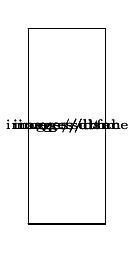
\begin{tikzpicture}
	\mode<beamer>{
    	  \uncover<1>{\pgftext[bottom,left,at={\pgfpointxy{2}{0}}]{\pgfuseimage{surface}};}
    	  \uncover<2>{\pgftext[bottom,left,at={\pgfpointxy{2}{0}}]{\pgfuseimage{dsm}};}
    	  \uncover<3>{\pgftext[bottom,left,at={\pgfpointxy{2}{0}}]{\pgfuseimage{dtmh}};}
    	  \uncover<4>{\pgftext[bottom,left,at={\pgfpointxy{2}{0}}]{\pgfuseimage{dtm}};}
    	  \uncover<5>{\pgftext[bottom,left,at={\pgfpointxy{2}{0}}]{\pgfuseimage{dtmn}};}
	}
	\mode<beamer:0>{
    	  \uncover<1>{\pgftext[bottom,left,at={\pgfpointxy{2}{0}}]{\pgfuseimage{surface}};}
    	  \uncover<2>{\pgftext[bottom,left,at={\pgfpointxy{2}{0}}]{\pgfuseimage{dsm}};}
    	  \uncover<3>{\pgftext[bottom,left,at={\pgfpointxy{2}{0}}]{\pgfuseimage{dtmh}};}
    	  \uncover<4>{\pgftext[bottom,left,at={\pgfpointxy{2}{0}}]{\pgfuseimage{dtm}};}
    	  \uncover<5>{\pgftext[bottom,left,at={\pgfpointxy{2}{0}}]{\pgfuseimage{dtmn}};}
	}
	\end{tikzpicture}
   \end{center}
\end{frame}
%%==================================================================S 
\subsection{Method}
%%==================================================================F 
\begin{frame}
    \frametitle{Vegetation filter}
    \begin{enumerate}
     \item Input data is the previous \emph{terrain} vs. \emph{object} classification (single and double pulse).
     \item Raster mask is created.
     \item<2-> It is possible searching for:
	\begin{itemize}
	 \item<2-> \alert<2>{buildings} $\Rightarrow$ cell value = 1 if at least one single object point lays in it
	 \item<3-> \alert<3>{vegetation} $\Rightarrow$ cell value = 1 if at leas one double terrain point lays in it
	 \item<4-> cell value = 0 otherwise
	\end{itemize}
    \end{enumerate}
\end{frame}
%%==================================================================F 
\begin{frame}
    \frametitle{Vegetation filter}
    \begin{enumerate}
	\item A region growing of the raster mask is used to feed a convex-hull algorithm.
	\uncover<2->{\item Dimensions and ratio between \alert<2>{area} and \alert<2>{perimeter} are used to classify segments
	  \begin{itemize}
	    \item Small or narrow shape objects are unlikely to be buildings.
	    \item Double terrain points are considered as vegetation.
	    \item Object double pulse outside hull segments are considered as vegetation.
	    \item Otherwise are buildings.
	  \end{itemize}}
    \end{enumerate}
\end{frame}
%%==================================================================Sb 
\subsection{Results}
%%==================================================================F
\pgfdeclareimage[height=7.5cm]{olbia_class}{images/olbia_veg_build}
\pgfdeclareimage[height=7.5cm]{olbia}{images/olbia}
\begin{frame}
    \frametitle{Olbia dataset}
    \begin{center}
      \begin{tikzpicture}
	  \pgftext[bottom,left,at={\pgfpointxy{0}{0}}]{\pgfuseimage{olbia}};
	  \uncover<2>{\pgftext[bottom,left,at={\pgfpointxy{0}{0}}]{\pgfuseimage{olbia_class}}}
      \end{tikzpicture}
    \end{center}
\end{frame}
%%==================================================================F
\begin{frame}
  \frametitle{Olbia confusion matrix}
  \begin{table}
    \begin{center} \resizebox{10cm}{!}{
      \begin{tabular}{llccccc}
	\toprule
	& & \multicolumn{4}{c}{\textbf{CLASSIFICATION}} & \\
	\cline{3-6}
	& & \multicolumn{2}{c}{\textbf{Buildings}} & \multicolumn{2}{c}{\textbf{Vegetation}} & \textbf{Total} \\
	\cline{3-6}
	& & Points & $\%$ & Points & $\%$ & \\
	\hline
	\multirow{3}{*}{\textbf{TRUE}} & \textbf{Buildings} & 179678 & 83.73 & 34919 & \alert{16.6} & 214597 \\
	& \textbf{Vegetation} & 37590 & \alert{7.5} & 388709 & 91.18 & 426299 \\
	& \textbf{Total} & 217268 & - & 423628 & - & 640896 \\
	\bottomrule
      \end{tabular}}
    \end{center}
  \end{table}
  \begin{enumerate}
    \item Type \texttt{I} error (Reject building points): \alert{$16.6\%$}
    \item Type \texttt{II} error (Accepting vegetation as buildings): \alert{$7.5\%$}
    \item Total error: \alert{$10.6\%$}
  \end{enumerate}
\end{frame}
%%==================================================================F 
\begin{frame}
  \frametitle{Vegetation filter problems}
    \begin{enumerate}
	\item Vegetation filtering is strongly affected by the pre-classification as terrain and off-terrain points.
	\item Some difficulties arise when trying to set filtering parameters for wide zones.
	\item Misclassified objects lead to:
	    \begin{itemize}
		\item High Type \texttt{I} error due to misclassified building edges.
		\item Type \texttt{II} error due to very dense vegetation wrongly classified as building or also elevated terrain zones misclassified as object and then later misclassfied as buildings.
	    \end{itemize}
    \end{enumerate}
\end{frame}
%%==================================================================F
\pgfdeclareimage[height=7.5cm]{olbia21_shade}{images/olbia_site21_shade}
\begin{frame}
  \frametitle{Vegetation classification in a small zone}
    \begin{center}
      \begin{tikzpicture}
	  \pgftext[bottom,left,at={\pgfpointxy{0}{0}}]{\pgfuseimage{olbia21_shade}};
      \end{tikzpicture}
    \end{center}
\end{frame}
%%==================================================================F
\begin{frame}
  \frametitle{Vegetation classification in a small zone}
  \begin{table}
    \begin{center} \resizebox{10cm}{!}{
      \begin{tabular}{llccccc}
        \toprule
        & & \multicolumn{5}{c}{\textbf{CLASSIFICATION}} \\
        \cline{3-7}
        & & \multicolumn{2}{c}{\textbf{Buildings}} & \multicolumn{2}{c}{\textbf{Vegetation}} & \textbf{Total} \\
        \cline{3-7}
        & & \footnotesize{Points} & \footnotesize{\%} & \footnotesize{Points} & \footnotesize{\%} & \footnotesize{Points} \\
        \hline\hline
        \multirow{3}{*}{\textbf{TRUE}} & \textbf{Buildings} & 14817 & 93.4 & 989 & \alert{6.3} & 15806 \\
        & \textbf{Vegetation} & 3001 & \alert{4.7} & 60444 & 95.3 & 63445 \\
        & \textbf{Total} & 17818 & - & 61433 & - & 79251 \\
        \bottomrule
      \end{tabular}}
    \end{center}
  \end{table}
  \begin{enumerate}
   \item Type \texttt{I} error: \alert{$6.3\%$}
   \item Type \texttt{II} error: \alert{$4.7\%$}
   \item Total error: \alert{$5\%$}
  \end{enumerate}
\end{frame}
%%==================================================================F
\pgfdeclareimage[height=5.5cm]{olbia21_errors}{images/olbia_site21_errors}
\begin{frame}
  \frametitle{Vegetation classification errors in a small zone}
  \begin{enumerate}
    \item Type \texttt{I} errors are due to few misclassified edges. 
    \item Type \texttt{II} errors are produced by stem parts placed over the river.
  \end{enumerate}
  \begin{center}
    \begin{tikzpicture}
	\pgftext[bottom,left,at={\pgfpointxy{0}{0}}]{\pgfuseimage{olbia21_errors}}
    \end{tikzpicture}
  \end{center}
\end{frame}
%%==================================================================Sb
\subsection{Conclusions}
%%==================================================================F 
\begin{frame}
  \frametitle{Vegetation filter conclusions}
    \begin{enumerate}
        \item A new tool for vegetation filtering able to distinguish between building and vegetation with only altimetric LiDAR data has been done.
	\item The filter starts from a first classification made with the built-in LiDAR filtering tools available in GRASS GIS 6.
	\item The filter makes use of dimensions and the ratio between area and perimeter of the previously classified objects.
	\item About the $90\%$ of the points are correctly classified into vegetation and buildings.
	    \begin{itemize}
		\item Wide vegetation regions are always correctly classified as well as the majority of single trees.
		\item Most of the building shapes are well defined.
	    \end{itemize}
    \end{enumerate}
\end{frame}
%%==================================================================S
\section{Conclusions}
%%==================================================================F 
\begin{frame}
    \frametitle{Final conclusions}
    \begin{enumerate}
     \item Two filters have been implemented and published as a built-in tool within the free and open source software (FOSS) GRASS GIS.
     \item The community has helped to improve the software in such a way to obtain a solid filter and improve the interpolation command.
     \item It has been proved that FOSS is a feasible way to use LiDAR programs without depending on proprietary software.
    \end{enumerate}
\end{frame}
%%==================================================================F 
\begin{frame}
    \frametitle{Future work}
    \begin{enumerate}
     \item Improvement in pre-classification into terrain and off-terrain
     \item Some efforts should be focused on enhancing edges misclassification as vegetation
     \item Some studies considering LiDAR intensity, multi-pulses information and roughness parameters
     \item Parallel jobs	
    \end{enumerate}
\end{frame}
%%==================================================================F  THE END
\againframe{portada}